\documentclass[10pt,letterpaper]{article}
\usepackage[utf8]{inputenc}
\usepackage{amsmath}
\usepackage{amsfonts}
\usepackage{amssymb}
\usepackage{graphicx}
\usepackage{algorithm}
\usepackage{algpseudocode}

\newcommand{\R}{\mathbb{R}}
\renewcommand{\thesubsection}{\thesection.\alph{subsection}}

\author{Brock Ellefson}
\title{CSCI432 HW5}

\begin{document}
\maketitle

\section{Prove that the Frechet distance is a distance metric}

Prove that the Frechet distance is a distance metric.\\
\\
To be a distance metric, you must satisfy 4 requirements:\\
Let X = discrete space\\
A metric is a function d: X x X $\rightarrow$ $\R$ such that:
\begin{enumerate}
  \item d(x,y) = d(y,x)
  \item d(x,y) = 0 $\Leftrightarrow$ x = y
  \item d(x,y) + d(y,z) $\geq$ d(x,z)
  \item d(x,y) $\geq$ 0
\end{enumerate}
So,\\
Let $A, B$ be two curves in a metric space, and t as a parameter in time. A and B are the infimum of all $\alpha$ and $\beta$ of [0,1] where t $\in$ [0,1]\\
Then the Frechet Distance is:\\
$F(A,B) = inf_{\alpha,\beta} max_{t\in[0,1]}\lbrace d(A(\alpha(t)),B(\beta(t)))\rbrace  $.\\
\\
So,\\
$F(A,B) = inf_{\alpha,\beta} max_{t\in[0,1]}\lbrace d(A(\alpha(t)),B(\beta(t)))\rbrace  $, and\\
$F(B,A) = inf_{\beta,\alpha} max_{t\in[0,1]}\lbrace d(B(\beta(t)),A(\alpha(t)))\rbrace  $.


\section{Recurrence Relations}
\subsection{T(n) = 2T(n/4) + n$^{2}$}
Master's Theorem:\\
T(n) = aT($\frac{n}{b}$) + f(n)\\
Where, a $\geq$ 1, b $>$ 1, f(n) is asymptotically positive\\
\\
T(n) = 2T(n/4) + n$^{2}$\\
a = 2, b = 4, f(n) = n$^{2}$\\
n$^{log_{b}a}$ $\Rightarrow$ n$^{log_{4}2}$ $\Rightarrow$ n$^{1/2}$\\
Case 3:\\
if f(n) is $\Omega$(n$^{log_{b}a + \epsilon}$) for some $\epsilon > 0$ and if f(n/b) $\leq$ f(n), then T(n) = $\theta(f(n))$\\
Therefore, T(n) = $\theta(n^{2})$

\subsection{T(n) = 4T(n/2) + n}
Master's Theorem:\\
T(n) = aT($\frac{n}{b}$) + f(n)\\
Where, a $\geq$ 1, b $>$ 1, f(n) is asymptotically positive\\
\\
T(n) = 4T(n/2) + n\\
a = 4, b = 2, f(n) = n\\
n$^{log_{b}a}$ $\Rightarrow$ n$^{log_{2}4}$ $\Rightarrow$ n$^{2}$\\
Case 1:\\
if f(n) = O(n$^{log_{b}a - \epsilon}$) for some $\epsilon > 0$ then T(n) = $\theta$( n$^{2}$).\\
Therefore, T(n) =  $\theta$( n$^{2}$)

\subsection{T(n) = 3T(2n/3) + 4n}
Master's Theorem:\\
T(n) = aT($\frac{n}{b}$) + f(n)\\
Where, a $\geq$ 1, b $>$ 1, f(n) is asymptotically positive\\
\\
T(n) = 3T(2n/3) + 4n\\
a = 3, b = 2/3, f(n) = 4n\\
n$^{log_{b}a}$ $\Rightarrow$ n$^{log_{3/2}3}$ $\Rightarrow$ n$^{2.71}$\\
Case 1:\\
if f(n) = $O(n^{log_{b}a - \epsilon})$ for some $\epsilon > 0$ then T(n) = $\theta(n^{2.71})$.\\
Therefore, T(n) =  $\theta(n^{2.71})$

\subsection{T(n) = T(n/2) + T(n/3)}

\begin{figure}[h]
	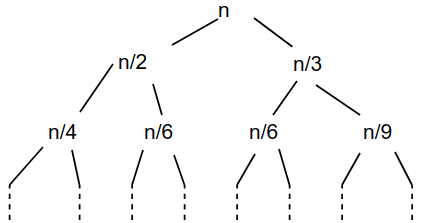
\includegraphics[scale = .25]{recurtree1hw5.png}
\end{figure}

\noindent Our longest path in this tree is the leftmost path, following a sequence: $log_{2}n$. So our initial guess is for this recurrence is $O(nlogn)$.\\
\\


\subsection{2T(n/2) + O(log n)}


\section{Climbing Stairs Problem}


\begin{algorithm}
\caption{Climbing Stairs}\label{euclid}
\begin{algorithmic}[1]
\State \textbf{Input:} n (number of stairs), k (max steps can advance at once)
\State \textbf{Output:} Integer (Numbers of ways to reach destination)

\State \textbf{Procedure:} $CountingStairs(n, k)$
\State count $\leftarrow$ 0
\If {n $\leq$ 1}
	\State \textbf{return} 1
\EndIf
\For{$i \leftarrow 1...(n)$} 
	\State $count \leftarrow COUNTINGSTAIRS(n-i, k)$
\EndFor
\State \textbf{return} count


\end{algorithmic}
\end{algorithm}


\end{document}